\subsection{Quantum Field Theory Axioms (A5--A6)}
%-----------------------------------------------------------------------------

\begin{tcolorbox}[colback=yellow!5, colframe=yellow!60!black, 
    title={\textbf{Conventions: Units, Masses, and Normalizations}}, fonttitle=\bfseries]

\textbf{Units and constants:}
\begin{itemize}[leftmargin=1.5em, topsep=2pt, itemsep=1pt]
    \item Natural units: $\hbar = c = 1$; energies in GeV, lengths in GeV$^{-1}$.
    \item Reference data: CODATA 2022, PDG 2024.
    \item Metric signature: $(+,-,-,-)$.
    \item Levi-Civita tensor: $\varepsilon^{0123} = +1$, $\tilde{F}^{\mu\nu} = \frac{1}{2}\varepsilon^{\mu\nu\rho\sigma}F_{\rho\sigma}$.
\end{itemize}

\textbf{Planck mass definitions:}
\begin{center}
\begin{tabular}{@{}lll@{}}
\toprule
\textbf{Symbol} & \textbf{Definition} & \textbf{Value}\\
\midrule
$M_{\mathrm{Pl}}$ (unreduced) & $G^{-1/2}$ & $1.221 \times 10^{19}$ GeV\\
$\Mpl$ (reduced) & $(8\pi G)^{-1/2}$ & $2.435 \times 10^{18}$ GeV\\
\bottomrule
\end{tabular}
\end{center}
\textbf{Convention:} Block formulas (Sec.~\ref{sec:e8}) use $M_{\mathrm{Pl}}$ (unreduced). 
Relation: $M_{\mathrm{Pl}} = \sqrt{8\pi}\,\Mpl$.

\textbf{Axion sector:}
\begin{itemize}[leftmargin=1.5em, topsep=2pt, itemsep=1pt]
    \item Axion field $a$: Dimensionless, $2\pi$-periodic. Physical field: $a_{\text{phys}} = f_a \cdot a$.
    \item Chern--Simons term: $\mathcal{L} \supset \cthree\, a\, F\tilde{F}$ with $\cthree = 1/(8\pi)$.
    \item Coupling: $\gagg = -4\cthree$ is dimensionless; $g_{a\gamma\gamma}^{\text{(phys)}} = \gagg / f_a$ has dimension $[\text{energy}]^{-1}$.
    \item \textbf{Maxwell convention:} We define the field strength by the exterior derivative $F := dA$, i.e.\ $F_{AB}=2\partial_{[A}A_{B]}$, independent of the torsionful affine connection (we do not use $F_{AB}=2\hat{\nabla}_{[A}A_{B]}$). Therefore U(1) gauge invariance is exact in the electromagnetic sector.
\end{itemize}
\end{tcolorbox}

\begin{axiom}{Axion--Photon Anomaly Coupling}{APC}
The unique additional coupling in the low-energy effective theory is a 
pseudoscalar axion--photon interaction of the form $\cthree\, a F\tilde{F}$, 
fixed by the abelian anomaly (Fujikawa method).

\tcblower
\textbf{Status:} Standard in anomaly physics; follows from chiral measure.

\textbf{Consequence:} The axion--photon coupling is
\begin{equation}
    \cthree = \frac{1}{8\pi}
\end{equation}
with no remaining normalization freedom.
\end{axiom}

\begin{axiom}{Modulus Closure in Background-Field Gauge}{BFG}
We introduce a dimensionless coupling modulus $\sigma$ with electromagnetic kinetic function
\begin{equation}
    \mathcal{L} \supset -\frac{1}{4} f(\sigma)\,F_{\mu\nu}F^{\mu\nu}
    + \frac{1}{2}(\partial\sigma)^2,
    \qquad 
    \alpha(\sigma)=\frac{1}{4\pi f(\sigma)}.
\end{equation}
The physical vacuum extremizes the effective action with respect to $\sigma$:
\begin{equation}
    \frac{\delta\Gamma_{\mathrm{eff}}}{\delta\sigma}=0.
\end{equation}
In background-field gauge, the effective potential can be written as
$V_{\mathrm{eff}}(\sigma)=U(\alpha(\sigma)) + V_{\mathrm{geo}}(\sigma)$, where
$V_{\mathrm{geo}}'(\sigma_\star)=0$ by geometric closure.
If $\alpha(\sigma)$ is monotonic near the vacuum, this is equivalent to
\begin{equation}
    \frac{\partial U}{\partial \alpha}=0,
    \qquad U(\alpha)=U(\sigma(\alpha)).
\end{equation}

\tcblower
\textbf{Status:} Standard in modulus stabilization; background-field gauge provides a clean definition of $\Gamma_{\mathrm{eff}}$.

\textbf{Consequence:} $\alpha$ is fixed by a modulus extremum, not treated as a variational constant.
\end{axiom}

%-----------------------------------------------------------------------------
\subsection{Closure Axioms (A7--A8)}
%-----------------------------------------------------------------------------

\begin{axiom}{Standard Model Hypercharge Trace}{SMT}
The hypercharge trace invariant, summed over all SM fermions with GUT normalization 
$(5/3)$, is:
\begin{equation}
    \bone = \frac{5}{3} \sum_{\text{SM fermions}} Y_f^2 = \frac{41}{10}
\end{equation}
In TFPT this quantity appears as the \emph{spectral quadratic index} of the
hypercharge-coupled boundary operators in the regulated determinant
(Appendix~\ref{app:boundary}), not as an RG flow coefficient.

\tcblower
\textbf{Status:} Direct consequence of SM particle content; independent of RG scale.

\textbf{Important distinction:} $\bone$ is a \emph{hypercharge trace invariant}, 
not the one-loop beta function coefficient $b_1^{(\text{RG})}$. While numerically 
identical, their physical roles differ:
\begin{itemize}[leftmargin=1.5em, topsep=2pt, itemsep=1pt]
    \item $b_1^{(\text{RG})}$: Controls energy dependence $d\alpha_1/d\ln\mu$
    \item $\bone$ (TFPT): Discrete index counting charge content; scale-independent
\end{itemize}

\textbf{Consequence:} No exotic particles or modified charge structure required.
\end{axiom}

\begin{tcolorbox}[colback=yellow!3, colframe=yellow!50!black, 
    title={\textbf{Scale Consistency: Why $\bone$ (UV) Determines $\alpha$ (IR)}}, fonttitle=\bfseries\small]
\textbf{Potential objection:} The abelian trace $\bone = 41/10$ is computed from the full SM spectrum 
(quarks, leptons, gauge bosons) at high energies. How can it determine $\alpha$ in the Thomson 
limit ($Q^2 \to 0$)?

\textbf{Resolution:} The CFE is a stationarity (closure) condition for the effective action; it is \emph{not} an RG differential equation.

\begin{enumerate}[leftmargin=1.5em, topsep=2pt, itemsep=1pt]
    \item \textbf{Spectral origin:} In the APS framework with flat $U(1)_Y$ holonomies on the boundary cycles,
        the regulated determinant produces a universal trace coefficient proportional to $\sum_f Y_f^2$.
        Thresholds affect non-universal finite terms, not this discrete spectral index.
    \item \textbf{Field-content fixed coefficient:} $\bone$ is the GUT-normalized hypercharge trace 
        $\frac{5}{3}\sum_f Y_f^2$ of the full SM spectrum. Once the field content and charge assignments are fixed, 
        $\bone$ is a discrete input and does not ``run'' as a function of $\mu$.
    \item \textbf{UV log coefficient, not IR running:} In the one-loop effective action, $\bone$ multiplies the UV logarithmic term 
        coming from the abelian charge trace. TFPT uses this UV coefficient inside the stationarity condition; it does not attempt to compute 
        the infrared running $\alpha(\mu)$.
    \item \textbf{Threshold independence (anomaly matching):} Below mass thresholds, particles decouple from IR loops, but the UV charge-trace 
        coefficient is fixed by the UV-complete spectrum. The sum $41/10$ is the asymptotic value and remains the relevant discrete input.
    \item \textbf{CFE vs.\ RG:} Standard RG asks ``how does $\alpha(\mu)$ evolve?'' The CFE asks ``what value of $\alpha$ makes the effective action stationary 
        given $(\cthree,\phiz,\bone)$?'' It is a closure condition, not a flow equation.
\end{enumerate}

\textbf{Reviewer-safe statement:} We use $\bone$ as the discrete spectral trace coefficient of the
hypercharge-coupled boundary operators in the UV logarithmic term of the regulated determinant.
TFPT explicitly does \emph{not} claim to compute the IR running $\alpha(\mu)$ or threshold matching.

\textbf{Prediction:} If additional charged particles exist beyond the SM (e.g., SUSY partners), 
$\bone$ would change and the CFE would predict a \emph{different} $\alpha$. This is testable.
\end{tcolorbox}

\begin{axiom}{GR Renormalization Condition}{GRN}
In the torsion-free limit ($K \to 0$), the theory must exactly reproduce 
Einstein--Hilbert gravity.

\tcblower
\textbf{Status:} Physical consistency requirement.

\textbf{Consequence:} Fixes the gravitational coupling structure:
$\kappa^2 = 8\pi G$, with the dimensionless ratio $\xi = \cthree/\phiz$ constrained by topology.
The dimensional scale $M_{\mathrm{Pl}}$ remains an external input.
\end{axiom}

%=============================================================================
\section{Derivation of Fundamental Constants}
%=============================================================================

%-----------------------------------------------------------------------------
\subsection{\texorpdfstring{The Geometric Scale $\phiz$}{The Geometric Scale phi0}}
%-----------------------------------------------------------------------------

\begin{theorem}{Existence and Uniqueness of $\phiz$}{phi0}
From Axioms A3 and A4, the geometric scale is uniquely determined:
\begin{equation}
    \phiz = \phitree + \deltatop = \frac{1}{6\pi} + \frac{3}{256\pi^4} = \num[round-mode=places,round-precision=17]{\TFPTvarphiZeroNum}
\end{equation}
\end{theorem}

\begin{proof}
From A3 ($\eta$-gluing): the M\"obius double cover contributes two physical boundary
cycles ($2\pi+2\pi$) plus a discrete seam gluing term ($2\pi$), giving
$R_{\text{total}}=6\pi$. The stationarity condition $\partial_\varphi V_{\text{eff}} = 0$
under the normalization $\chi = \varphi R = 1$ yields $\phitree = 1/(6\pi)$.

From A4: the unique gauge-invariant correction at leading order is 
$\deltatop = 48\cthree^4 = 3/(256\pi^4)$.
\end{proof}

\begin{tcolorbox}[colback=gray!5, colframe=gray!60, breakable,
    title={\textbf{Dictionary: $\beta_{\text{rad}}$ and Canonical Consequences}}, fonttitle=\bfseries\small]
\textbf{Definition (notation):}
\[
\beta_{\text{rad}} := \frac{\phiz}{4\pi}.
\]
\textit{Note:} dimensionless; equals the birefringence angle in radians for the minimal topological excursion $\Delta a_{\text{top}}=\phiz$.

\textbf{Immediate algebraic consequences:}
\begin{equation}
    \phiz = 4\pi\beta_{\text{rad}}, 
    \qquad 
    \beta_{\text{deg}} := \frac{180}{\pi}\,\beta_{\text{rad}}.
\end{equation}
\begin{equation}
    \gagg = -4\cthree = -\frac{1}{2\pi},
    \qquad
    \deltatop = 48\cthree^4 = \frac{3}{256\pi^4}.
\end{equation}

\textbf{Remark:} Many later ``$\beta_{\text{rad}}$-centric'' relations are compact rewrites of earlier definitions. 
We catalogue their logical status (definition vs.\ consequence vs.\ lemma vs.\ prediction) in Appendix~\ref{app:identities}.
\end{tcolorbox}

% Suite-extracted invariant table (high precision)
\TFPTCoreInvariantTable

%-----------------------------------------------------------------------------
\subsection{The Cubic Fixed-Point Equation (CFE)}
%-----------------------------------------------------------------------------

\begin{definition}{Effective Potential Parameters}{params}
From the 11D Chern--Simons reduction (A5) and modulus-closure structure (A6):
\begin{align}
    A &= 2\cthree^3 = \frac{1}{256\pi^3} \approx 1.2598 \times 10^{-4}\\[0.5em]
    \mathcal{K} &= \frac{\bone}{2\pi}\ln\frac{1}{\phiz} \approx 1.9147
\end{align}
\textbf{Notation:} We use $\mathcal{K}$ (calligraphic) for this CFE parameter to 
distinguish it from $\kappa^2 = 8\pi G$ (gravitational coupling).
\end{definition}

\begin{tcolorbox}[colback=gray!5, colframe=gray!60,
    title={\textbf{Lemma (Geometric Fixing of the Log)}}, fonttitle=\bfseries\small]
In TFPT the one-loop logarithm is the ratio of a UV scale to a geometrically fixed IR scale:
\begin{equation}
    \ln\frac{1}{\phiz} = \ln\frac{\Lambda}{\mu_{\text{geo}}}.
\end{equation}
Here $\mu_{\text{geo}} \equiv \ell_{\text{geo}}^{-1}$ is fixed by the M\"obius curvature
normalization ($R_{\text{total}}=6\pi$), and $\phiz = \ell_{\text{UV}}/\ell_{\text{geo}}$.
Thus the renormalization point is not a free choice but is geometrically determined.
\end{tcolorbox}

\begin{theorem}{Cubic Fixed-Point Equation}{CFE}
From Axioms A5--A7 and the modulus-closure condition (A6), the vacuum extremum
$\delta\Gamma_{\mathrm{eff}}/\delta\sigma=0$ is equivalent to $\partial U/\partial\alpha = 0$
and yields the cubic fixed-point equation:
\begin{equation}
    \boxed{\alpha^3 - 2\cthree^3\,\alpha^2 - 8\bone\cthree^6\ln\frac{1}{\phiz(\alpha)} = 0}
    \label{eq:CFE}
\end{equation}
This equation has exactly one positive real root.
\end{theorem}

\begin{proof}
In background-field gauge, the one-loop effective potential takes the form
\begin{equation}
    U(\alpha) = \frac{A}{4}\alpha^4 - \frac{2}{3}A\cthree^3\alpha^3 - 8A\bone\cthree^6 L\,\alpha + \ldots
\end{equation}
where $L = \ln(1/\phiz)$. The modulus-closure condition 
$\delta\Gamma_{\mathrm{eff}}/\delta\sigma = 0$ reduces to $\partial U/\partial\alpha = 0$
(monotonic $\alpha(\sigma)$), giving
\begin{equation}
    A\bigl[\alpha^3 - 2\cthree^3\alpha^2 - 8\bone\cthree^6 L\bigr] = 0
\end{equation}
(The factor 2 arises from differentiating the $2/3$ coefficient of the cubic term.)
For $A \neq 0$, this is the CFE. Descartes' rule of signs guarantees exactly 
one positive real root.
\end{proof}

\begin{figure}[H]
\centering
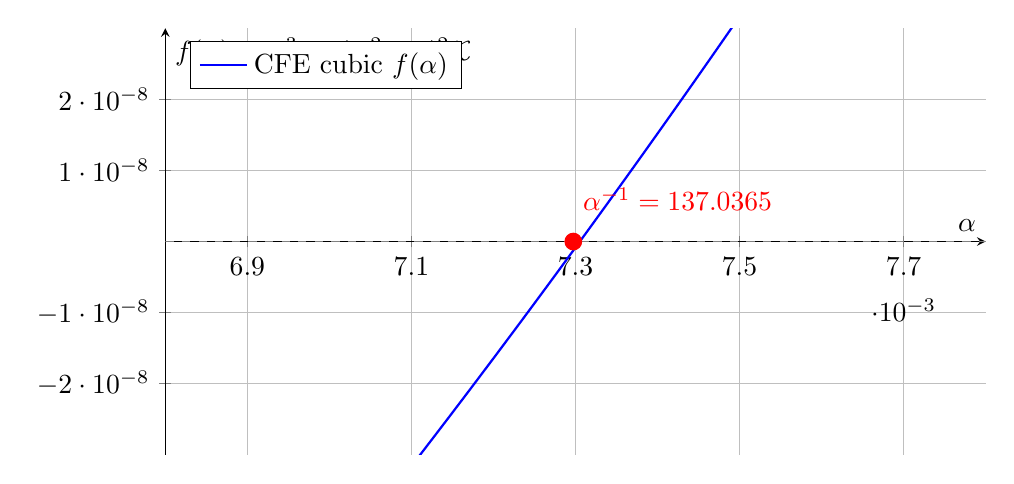
\begin{tikzpicture}
\begin{axis}[
    width=12cm, height=7cm,
    xlabel={$\alpha$},
    ylabel={$f(\alpha) = \alpha^3 - A\alpha^2 - A\cthree^2\mathcal{K}$},
    xmin=0.0068, xmax=0.0078,
    ymin=-3e-8, ymax=3e-8,
    grid=major,
    axis lines=middle,
    xtick={0.0069, 0.0071, 0.0073, 0.0075, 0.0077},
    ytick={-2e-8, -1e-8, 0, 1e-8, 2e-8},
    scaled y ticks=false,
    yticklabel style={/pgf/number format/sci},
    legend pos=north west
]
    % CFE cubic
    \addplot[domain=0.0068:0.0078, samples=200, thick, blue] 
        {x^3 - 2*0.039788735773^3*x^2 - 8*4.1*0.039788735773^6*2.9439};
    \addlegendentry{CFE cubic $f(\alpha)$}
    
    % Root marker
    \addplot[only marks, mark=*, mark size=3pt, red] 
        coordinates {(0.00729733, 0)};
    \node[red, above right] at (axis cs:0.00729733, 0.3e-8) 
        {$\alpha^{-1} = 137.0365$};
    
    % Zero line
    \addplot[domain=0.0068:0.0078, dashed, gray] {0};
\end{axis}
\end{tikzpicture}
\caption{The CFE has a unique positive root at $\alpha \approx 0.007297$, 
corresponding to $\alpha^{-1} \approx 137.0365$ (baseline with fixed $\phiz$).}
\label{fig:CFE}
\end{figure}

\begin{figure}[H]
\centering
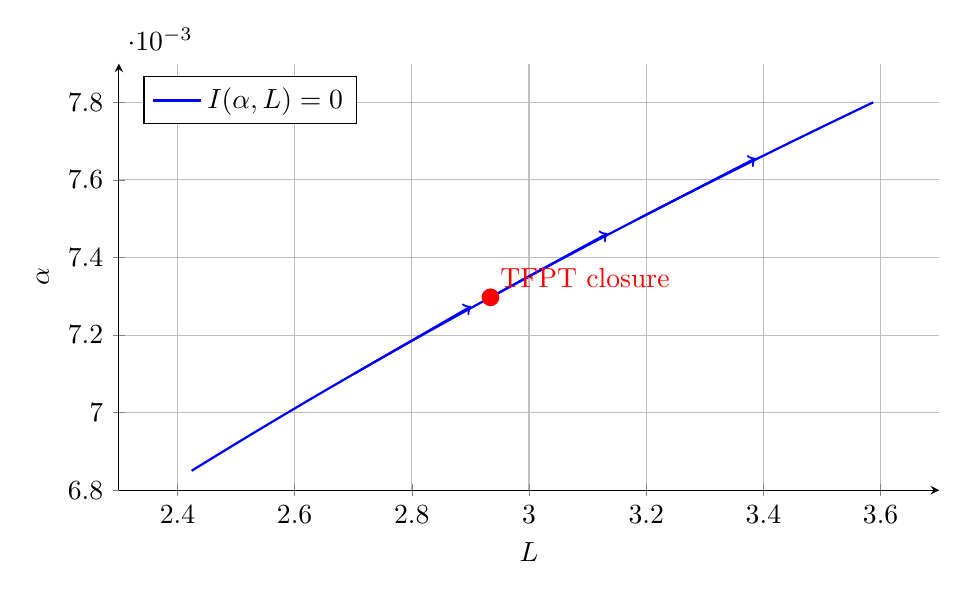
\begin{tikzpicture}
\begin{axis}[
    width=12cm, height=7cm,
    xlabel={$L$},
    ylabel={$\alpha$},
    xmin=2.3, xmax=3.7,
    ymin=0.0068, ymax=0.0079,
    grid=major,
    axis lines=left,
    legend pos=north west
]
    % Invariant surface I(\alpha,L)=0 (parametric form L(\alpha),\alpha)
    \addplot[domain=0.00685:0.0078, samples=240, thick, blue]
        ({(x^3 - 2*0.039788735773^3*x^2)/(8*4.1*0.039788735773^6)}, {x});
    \addlegendentry{$I(\alpha,L)=0$}

    % Flow direction from implicit differentiation: d\alpha/dL
    \addplot[->, thick, blue] coordinates {(2.701252,0.00710000) (2.901252,0.00727418)};
    \addplot[->, thick, blue] coordinates {(2.934229,0.00729733) (3.134229,0.00746216)};
    \addplot[->, thick, blue] coordinates {(3.187073,0.00750000) (3.387073,0.00765600)};

    % TFPT closure point (baseline)
    \addplot[only marks, mark=*, mark size=3pt, red] coordinates {(2.934224,0.00729733)};
    \node[red, above right] at (axis cs:2.934224,0.00729733) {TFPT closure};
\end{axis}
\end{tikzpicture}
\caption{Structural flow on the invariant surface $I(\alpha,L)=0$ in the $(L,\alpha)$ plane,
with arrows indicating $d\alpha/dL$ from implicit differentiation.
The marked point shows the TFPT closure solution.}
\label{fig:invariant_flow}
\end{figure}

%-----------------------------------------------------------------------------
\subsection{Geometric Self-Consistency (Backreaction)}
%-----------------------------------------------------------------------------

